\documentclass[../main.tex]{subfiles}
\begin{document}

\begin{figure}
    \centering
    \begin{subfigure}[b]{0.48\textwidth}
        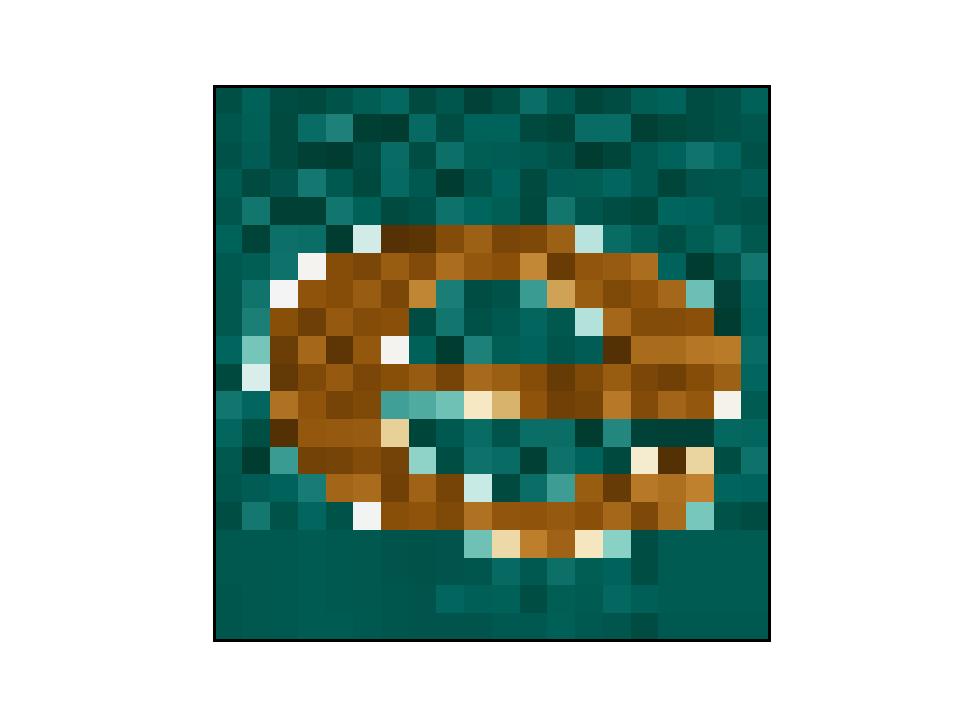
\includegraphics[width=\textwidth]{figures/pp/raw}
        \caption{Raw image.}
        \label{fig:gull}
    \end{subfigure}
    ~ %add desired spacing between images, e. g. ~, \quad, \qquad, \hfill etc. 
      %(or a blank line to force the subfigure onto a new line)
    \begin{subfigure}[b]{0.48\textwidth}
        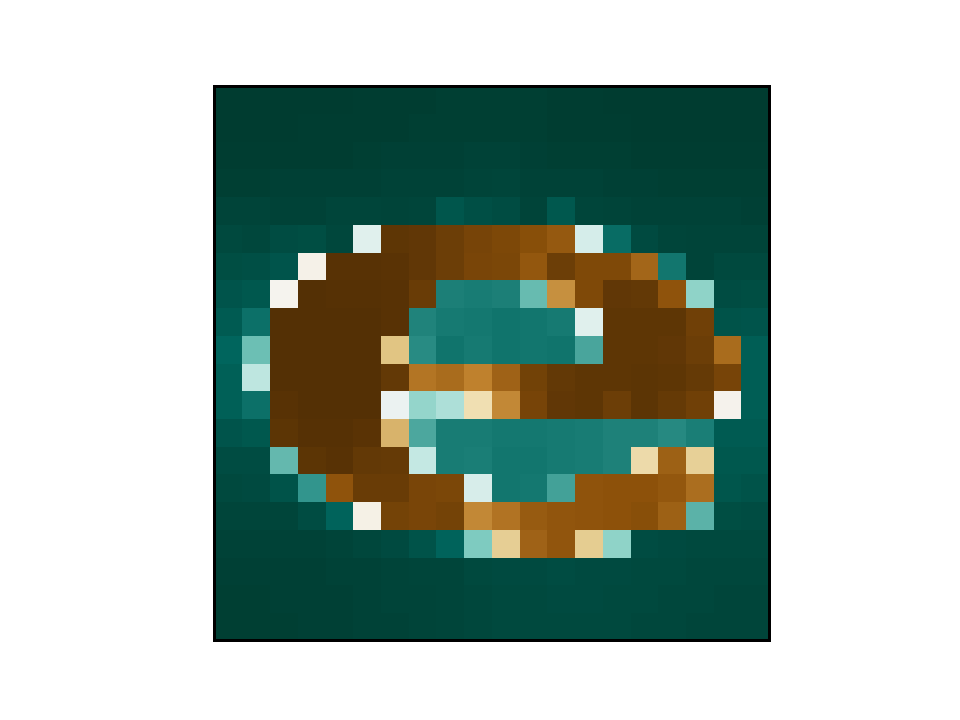
\includegraphics[width=\textwidth]{figures/pp/denoise}
        \caption{Denoised image.}
        \label{fig:denoise}
    \end{subfigure}
    ~ %add desired spacing between images, e. g. ~, \quad, \qquad, \hfill etc. 
    %(or a blank line to force the subfigure onto a new line)
    \begin{subfigure}[b]{0.48\textwidth}
        
\includegraphics[width=\textwidth]{figures/pp/img_to_bool}
        \caption{Binary image.}
        \label{fig:bool}
    \end{subfigure}
        ~ %add desired spacing between images, e. g. ~, \quad, \qquad, \hfill etc. 
    %(or a blank line to force the subfigure onto a new line)
    \begin{subfigure}[b]{0.48\textwidth}
        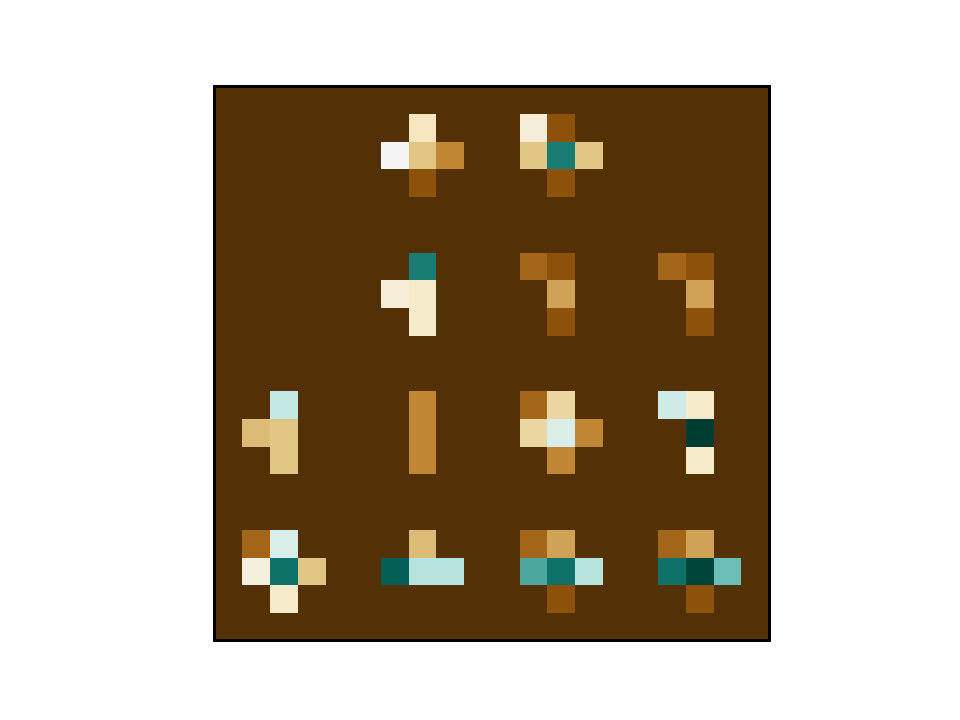
\includegraphics[width=\textwidth]{figures/pp/hog}
        \caption{Histogram of Oriented Gradients.}
        \label{fig:hog}
    \end{subfigure}
    \caption{Example of random selected image before and after preprocessing. The colors has been altered using a color map to visually enhance variance.}\label{fig:pp_image}
\end{figure}

In this section, the preprocessing of the images are shown. The preprocessing is preformed to enable easier classification for the classifier. As two different classifier approaches are examined in this report, it will also explain two different setups with feature engineering.

\subsection{Feature engineering for k-Nearest Neighbor Classifier}

Several different preprocessing tools were explored to make the character easier to recognize for the classifier. The first preprocessing tool applied was total-variation denoising on n-dimensional images \cite{dnoise_tv_chambolle}. This technique reduces the total variation of an image. This is useful to avoid classifying noise, as the picture will now contain fewer components with high spacial frequency. An example of this denoising technique is shown in the image \autoref{fig:denoise}.

To increase contrast, we used Otsu's method, which is a way to perform image thresholding based on clustering \cite{otsu} automatically. After thresholding, the image was morphologically closed. This is a standard technique in image processing to remove small wholes in binary images. The result is shown in \autoref{fig:bool}. All though the result was visually pleasing; it did not decrease the error rate. Therefore, this method was discarded from further analysis.

\subsubsection{Principal component analysis}

It is a substaintian challange and computationally heavy to preform classification on high dimentional data. Therefore, a dimention reduction tool is preferable before performing a k-Nearest Neighbor Classifier. In this project, the Principal Component Analysis procedure was used for reducing the number of correlated dimentions down to a set of linearly uncorrelated principle component. The optimal condition for the k-Nearest Neighbor Classifier is when PCA is used to reduce the dimention down to \vari{n_pca}.

\end{document}